% To whoever is reading this, this is sadly not I wrote during the exam. It could've been better during the exam HAHAHA

\documentclass{article}
\usepackage[a4paper, total={7in, 9.5in}]{geometry}
\usepackage[utf8]{inputenc}
\usepackage{amsmath}
\usepackage{amssymb}
\usepackage{multirow}
\usepackage{mathtools}
\usepackage{xfrac}

\DeclarePairedDelimiterX{\infdivx}[2]{(}{)}{%
  #1\;\delimsize\|\;#2%
}
\newcommand{\infdiv}{D\infdivx}
\DeclarePairedDelimiter{\norm}{\lVert}{\rVert}

\makeatletter
\renewcommand*\env@matrix[1][*\c@MaxMatrixCols c]{%
  \hskip -\arraycolsep
  \let\@ifnextchar\new@ifnextchar
  \array{#1}}
\makeatother

\title{MA2104 Suggested Solutions}
\author{Written by: Nicholas Russell Saerang\\Audited by: Chow Yong Lam}
\date{Semester 2, AY2021/2022\\Last Updated: \today}

\begin{document}

\maketitle

\begin{enumerate}
    \item Note that $S$ is a graph of a function $g(x,y)=4-4x-2y$, where $(x,y) \in D=[0,1]^2$. Therefore,
    \begin{align*}
        \iint_S f(x,y,z) \hspace{1mm}dS &= \iint_D f(x,y,g(x,y)) \sqrt{g_x^2 + g_y^2 + 1} \hspace{1mm}dA \\
        &= \iint_D f(x,y,g(x,y)) \sqrt{(-4)^2 + (-2)^2 + 1} \hspace{1mm}dA \\
        &= \sqrt{21} \iint_D f(x,y,g(x,y)) \hspace{1mm}dA \\
        &\approx \sqrt{21}\sum_{(x^*, y^*)} f(x^*, y^*, g(x^*,y^*)) \Delta x \Delta y \\
        &= \sqrt{21}(3-1+2+7)\cdot\frac{1}{2}\cdot\frac{1}{2} = \frac{11\sqrt{21}}{4}.
    \end{align*}
    %Fix - Russell
    Here, $\sum_{(x^*, y^*)}$ is basically summing over the four points provided in the question.
    
    \begin{center}
        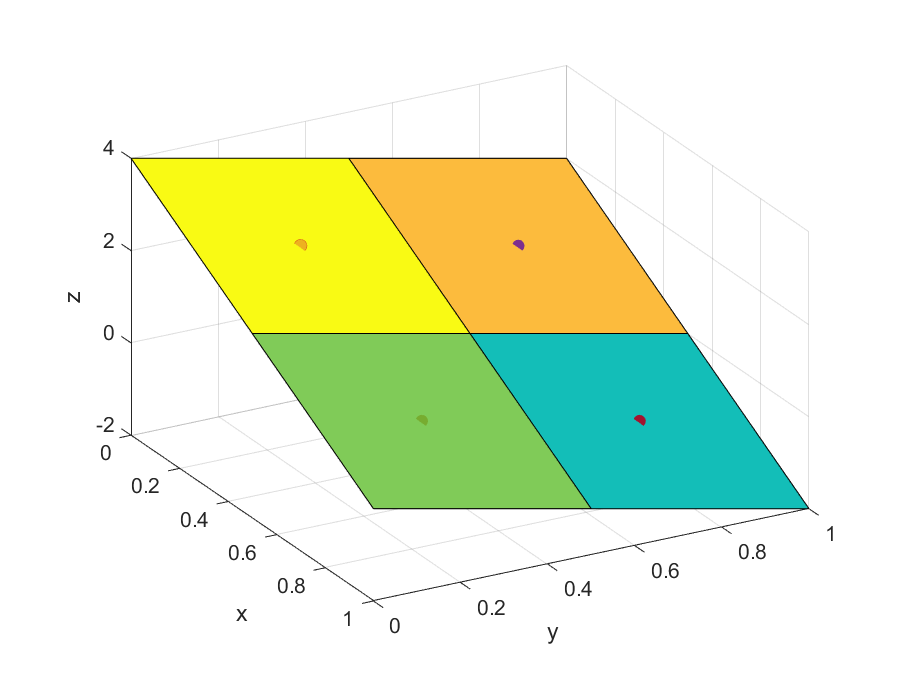
\includegraphics[scale=0.7]{q1.eps}
    \end{center}
    \newpage
    
    %Not sure if the summation subscript is clear/explanatory enough to show that it's including the 4 centers of the 0.5x0.5 squares. -YL
    
    \item Suppose $\textbf{F}(x,y) = \begin{pmatrix} X(x,y) \\ Y(x,y) \end{pmatrix}$. Since $X_y = Y_x = 3x^2 + 2y$, $\textbf{F}$ is conservative.\\
    %Fix - Russell
    Also, a possible potential function is $f(x,y) = x^3y + xy^2 + \frac{1}{3}y^3 - \frac{1}{4}\cos{2x}$. This is because we have
    \begin{align*}
        f(x,y) &= \int 3x^2y + \sin{x}\cos{x} + y^2 \hspace{1mm}dx\\
        &= x^3y - \frac{1}{4}\cos{2x} + xy^2 + p(y)\\
        f(x,y) &= \int x^3 + 2xy + y^2 \hspace{1mm}dy\\
        &= x^3y + xy^2 + \frac{1}{3}y^3 + q(x)
    \end{align*}
    for some function $p(y)$ and $q(x)$, to which we can set them to be $\frac{1}{3}y^3$ and $- \frac{1}{4}\cos{2x}$, respectively.\\
    Therefore,
    \begin{align*}
        \int_\textbf{C} \textbf{F}\cdot d\textbf{r} &= f(0, -\pi^2) - f(-\pi, 0)\\
        &= \left(-\frac{1}{3}\pi^6 - \frac{1}{4}\right) - \left(-\frac{1}{4}\right) = -\frac{1}{3}\pi^6.
    \end{align*}
    
    % Would be great to include the steps showing how to derive the potential function? -YL
    \vspace{2cm}
    \item Since $\text{comp}_{\textbf{n}(t)}\textbf{F}(R(t)) = \sqrt{1 - t^2}$ and $\norm{\textbf{F}} = 1$, using the fact that $\textbf{n}(t)$ are perpendicular to $R'(t)$, we must have $\text{comp}_{R'(t)}\textbf{F}(R(t)) = t$. You can take a look at the diagram below for the visualization. 
    %Fix - Russell
    \begin{center}
        \includegraphics[scale=0.5]{q3.png}
    \end{center}
    Thus,
    \begin{align*}
        \int_\textbf{C} \textbf{F}\cdot d\textbf{r} &= \int_0^1 \textbf{F}(R(t))\cdot R'(t) \hspace{1mm}dt\\
        &= \int_0^1 \text{comp}_{R'(t)}\textbf{F}(R(t)) \cdot \norm{R'(t)} \hspace{1mm}dt\\
        &= \int_0^1 t\sqrt{1^2 + (2t)^2 + (6t)^2} \hspace{1mm}dt\\
        % Would this times symbol be mixed up with cross product? Maybe it's only me. If it's not confusing to y'all (JB halp) then ignore this comment. -YL
        &= \int_0^1 t\sqrt{40t^2 + 1} \hspace{1mm}dt\\
        &=\frac{(40+1)^{\frac{3}{2}}}{120} - \frac{(1)^{\frac{3}{2}}}{120} = \frac{41\sqrt{41}-1}{120}.
        % Denominator should be 120? -YL
        % Not sure if the first 2 lines is clear/explanatory enough? Would a diagram be necessary (It could be me being too naggy ngl take my suggestions with a grain of salt plz) -YL
    \end{align*}
    
    %Fix - Russell
    \newpage
    \item Since $f(x,y)=f(x,-y)$, then
    \[\int_0^1 f(x,y) dy = \int_{-1}^0 f(x,y) dy = \frac{1}{2} \int_{-1}^1 f(x,y) dy\]
    Therefore,
    \begin{align*}
        &\int_0^2 \int_{-2}^2 f(x,y) dxdy\\
        &= \int_1^2 \int_{-2}^2 f(x,y) dxdy + \int_0^1 \int_{-2}^1 f(x,y) dxdy + \int_0^1 \int_{1}^2 f(x,y) dxdy\\
        &= \int_1^2 \int_{-2}^2 f(x,y) dxdy + \int_{-2}^1 \int_0^1 f(x,y) dydx + \int_{1}^2 \int_0^1 f(x,y) dydx\\
        &= \int_1^2 \int_{-2}^2 f(x,y) dxdy + \frac{1}{2}\int_{-2}^1 \int_{-1}^1 f(x,y) dydx + \int_{1}^2 \int_{-1}^0 f(x,y) dydx\\
        &= 1 + \frac{1}{2}\int_{-1}^1 \int_{-2}^1 f(x,y) dxdy + \int_{-1}^0 \int_{1}^2 f(x,y) dxdy\\
        &= 1 + \frac{1}{2}\cdot 6 + \frac{1}{3} = \frac{13}{3}.
    \end{align*}
    
    % Do we need to at least show the integral from 0 to 1 (w.r.t y) is equal to integral from -1 to 0 (w.r.t y)? -YL
    
    \vspace{2cm}
    \item Since $0 \le z \le 1 - |x|$, we have $|x| \le 1 - z \rightarrow z - 1 \le x \le 1 - z$ while $0 \le z \le 1$. Thus,
    \[\int_{-1}^1\int_0^{1-x^2}\int_0^{1-|x|}f(x,y,z)\hspace{1mm}dzdydx = \int_{0}^1\int_{z-1}^{1-z}\int_0^{1-x^2}f(x,y,z)\hspace{1mm}dydxdz.\]
    \begin{center}
        \includegraphics[scale=0.75]{q5.png}
    \end{center}
    
    \newpage
    \item Using the spherical coordinate transformation, we have $(x,y,z) = (\rho\cos\theta\sin\phi, \rho\sin\theta\sin\phi, \rho\cos\phi)$ and
    %Fix - Russell
    \[f(x,y,z)=\begin{cases}
        \frac{1}{10(1+\rho^3)},& \text{ if } \rho \le k\\
        0, &\text{ otherwise}
    \end{cases}\]
    
    % Minor detail: The function is still piecewise after the transformation and I think it's safer to keep that detail.
    
    \begin{enumerate}
        \item[(a)] We must have
        \begin{align*}
            1 &= \int_0^\pi \int_0^{2\pi} \int_0^k \frac{1}{10(1+\rho^3)} \rho^2\sin\phi\hspace{1mm}d\rho d\theta d\phi\\
            &= \int_0^\pi \int_0^{2\pi} \frac{\ln{(1+k^3)}}{30} \sin\phi\hspace{1mm}d\theta d\phi\\
            &= \frac{\pi}{15}\ln{(1+k^3)} \int_0^\pi \sin\phi\hspace{1mm}d\phi\\
            &= \frac{2\pi}{15}\ln{(1+k^3)}.
        \end{align*}
        Therefore, $k=\sqrt[3]{e^\frac{15}{2\pi} - 1}$.
        \vspace{1cm}
        \item[(b)] Note that
        \[z=\sqrt{x^2+y^2} \Rightarrow \phi=\frac{\pi}{4}\]\[\sqrt{(x^2+y^2+z^2)^3}+1=e^\frac{z}{\sqrt{x^2+y^2+z^2}} \Rightarrow \rho^3 + 1 = e^{\cos\phi} \Rightarrow \rho = \sqrt[3]{e^{\cos\phi} - 1}\]
        Also, since $\rho \le \sqrt[3]{e^{\cos\phi} - 1} \le \sqrt[3]{e - 1} < k$, all the points inside the region will % add "in the region"? -YL
        have a nonzero $f$-value. So this question boils down to evaluating the following integral.
        \begin{align*}
            &\int_0^{\frac{\pi}{4}} \int_0^{2\pi} \int_0^{\sqrt[3]{e^{\cos\phi} - 1}} \frac{1}{10(1+\rho^3)} \rho^2\sin\phi\hspace{1mm}d\rho d\theta d\phi\\
            &= \int_0^{\frac{\pi}{4}} \int_0^{2\pi} \frac{\sin\phi\cos\phi}{30} \hspace{1mm}d\theta d\phi\\
            &= \int_0^{\frac{\pi}{4}} \frac{2\pi\sin\phi\cos\phi}{30} \hspace{1mm}d\phi\\
            &= \int_0^{\frac{\pi}{4}} \frac{\pi\sin{2\phi}}{30} \hspace{1mm}d\phi\\
            &= \frac{\pi}{30}\cdot\frac{-1}{2}\cdot(\cos\frac{\pi}{2}-\cos 0) = \frac{\pi}{60}.
        \end{align*}
    \end{enumerate}
    
    \newpage
    \item
    \begin{enumerate}
        \item[(a)] Let $(u, v) = (x-2y, 2x+y)$. Thus $(x,y)=\left(\frac{u+2v}{5}, \frac{v-2u}{5}\right)$ and $\left\vert\frac{\partial(x,y)}{\partial(u,v)}\right\vert=\begin{vmatrix}\frac{1}{5} & \frac{2}{5} \\ -\frac{2}{5} & \frac{1}{5}\end{vmatrix}=\frac15$.\\
        Note that $5x^2+5y^2+1=u^2+v^2+1$. Suppose $(u, v) \in S=[-1,2]\times[0,3]$, then by the 2D-Jacobian we have
        \begin{align*}
            \iint_R f(x,y) \hspace{1mm}dA &= \iint_S f(x(u,v), y(u, v))\left\vert\frac{\partial(x,y)}{\partial(u,v)}\right\vert \hspace{1mm}dudv\\
            %Fix - Russell, also skill issue smh
            &= \frac15\iint_S (u^2+v^2+1) \hspace{1mm}dudv\\
            &= \frac15\int_0^3\int_{-1}^2 (u^2+v^2+1) \hspace{1mm}dudv\\
            &= \frac15\int_0^3\int_{-1}^2 (u^2+v^2) \hspace{1mm}dudv + \frac15(3-0)(2+1) \hspace{1 cm} \text{(take 1 out and it becomes the area)}\\
            &= \frac15\int_0^3 \left(\frac{2^3+1^3}{3}+(2+1)v^2\right) \hspace{1mm}dv + \frac95\\
            &= \frac35\int_0^3 (v^2+1) \hspace{1mm}dv + \frac95\\
            &= \frac35\left(\frac{3^3-0^3}{3}+(3-0)\right)+ \frac95 = 9.
            % Incorrect integration. Should be 3v^2 + 3 (with no outer coefficient) in the second to last line. Then the integration step w.r.t. is also affected. Final answer IS 45 though. -YL
        \end{align*}
        
        % Changed notation: \delta --> \partial -YL
        \vspace{1cm}
        \item[(b)] Note that along the path, $x^2+y^2=4$ is constant, so the average depth is just the constant value of $f(x,y)$ which is 21.
        
        \vspace{1cm}
        \item[(c)] We can parameterize the path as $R(t) = (-2\cos t, 2\sin t) , 0\le t \le \pi \Rightarrow R'(t) = (2\sin t, 2\cos t)$.\\
        The work done by the ocean is
        \begin{align*}
            \int_0^\pi \textbf{F}(x(t), y(t))\cdot R'(t) \hspace{1mm}dt &= \int_0^\pi \begin{pmatrix} 4\cos^2 t \\ 4\sin^2 t \end{pmatrix} \cdot \begin{pmatrix} 2\sin t \\ 2\cos t \end{pmatrix} \hspace{1mm}dt\\
            &= \int_0^\pi 8\sin t\cos^2 t + 8\cos t\sin^2 t \hspace{1mm}dt\\
            &= \left[\frac{8}{3}(\sin^3 t - \cos^3 t)\right]_0^\pi\\
            &= \frac{8}{3} + \frac{8}{3} = \frac{16}{3}.
        \end{align*}
    \end{enumerate}
    
    \newpage
    \item
    \begin{enumerate}
        \item[(a)] Suppose $\textbf{F}(x,y) = \begin{pmatrix} X(x,y,z) \\ Y(x,y,z) \\ Z(x,y,z) \end{pmatrix}$. Since $xz = X_y \neq Y_x = -2xy$, $\textbf{F}$ is not conservative.
        \vspace{1cm}
        %Fix - Russell
        \item[(b)] In the diagram below, the black point is the origin, while the yellow and cyan cubes represent E and E' respectively.
        \begin{center}
            \includegraphics[scale=0.5]{q8b.png}
        \end{center}
        The flux across \textbf{S} is just the overall flux across the surfaces of E, call this \textbf{T}, minus the total flux on the three sides of E', highlighted in brown. Suppose we denote the sides $\textbf{S}_1$, $\textbf{S}_2$, and $\textbf{S}_3$, where each side lies on the $xy$-plane, $xz$-plane, and the $yz$-plane, respectively. Note that by Gauss' Theorem,
        \begin{align*}
            \iint_\textbf{S} \textbf{F}\cdot \hspace{1mm}d\textbf{S} &= \iint_\textbf{T} \textbf{F}\cdot \hspace{1mm}d\textbf{T} - \left(\iint_{\textbf{S}_1} \textbf{F}\cdot \hspace{1mm}d\textbf{S}_1 + \iint_{\textbf{S}_2} \textbf{F}\cdot \hspace{1mm}d\textbf{S}_2 + \iint_{\textbf{S}_3} \textbf{F}\cdot \hspace{1mm}d\textbf{S}_3\right)\\
            &= \iiint_E \text{div }\textbf{F} \hspace{1mm}dV - \left(\iint_{\textbf{S}_1} \textbf{F}\cdot \hspace{1mm}d\textbf{S}_1 + \iint_{\textbf{S}_2} \textbf{F}\cdot \hspace{1mm}d\textbf{S}_2 + \iint_{\textbf{S}_3} \textbf{F}\cdot \hspace{1mm}d\textbf{S}_3\right)\\
            &= \iiint_E (yz - x^2 + 1 + x^2 - yz) \hspace{1mm}dV - \left(\iint_{\textbf{S}_1} \textbf{F}\cdot \hspace{1mm}d\textbf{S}_1 + \iint_{\textbf{S}_2} \textbf{F}\cdot \hspace{1mm}d\textbf{S}_2 + \iint_{\textbf{S}_3} \textbf{F}\cdot \hspace{1mm}d\textbf{S}_3\right)\\
            &= \iiint_E dV - \left(\iint_{\textbf{S}_1} \textbf{F}\cdot \hspace{1mm}d\textbf{S}_1 + \iint_{\textbf{S}_2} \textbf{F}\cdot \hspace{1mm}d\textbf{S}_2 + \iint_{\textbf{S}_3} \textbf{F}\cdot \hspace{1mm}d\textbf{S}_3\right)\\
            &= 1 - \left(\iint_{\textbf{S}_1} \textbf{F}\cdot \hspace{1mm}d\textbf{S}_1 + \iint_{\textbf{S}_2} \textbf{F}\cdot \hspace{1mm}d\textbf{S}_2 + \iint_{\textbf{S}_3} \textbf{F}\cdot \hspace{1mm}d\textbf{S}_3\right).\\
        \end{align*}
        For $\textbf{S}_1$, the normal vector is $-\textbf{k}$ but $z = 0$, so $\iint_{\textbf{S}_1} \textbf{F}\cdot \hspace{1mm}d\textbf{S}_1 = 0$. Similarly, for $\textbf{S}_2$, the normal vector is $-\textbf{j}$ but $y = 0$, so $\iint_{\textbf{S}_2} \textbf{F}\cdot \hspace{1mm}d\textbf{S}_2 = 0$. For $\textbf{S}_3$, the normal vector is $-\textbf{i}$ and $x = 0$. However, the dot product is non-zero, which is
        \begin{align*}
            \iint_{\textbf{S}_3} \textbf{F}\cdot \hspace{1mm}d\textbf{S}_3 &= \int_0^\frac{1}{2}\int_0^\frac{1}{2}\textbf{F}\cdot\begin{pmatrix}-1\\0\\0\end{pmatrix}dydz\\
            &= \int_0^\frac{1}{2}\int_0^\frac{1}{2}(-xyz-1)\hspace{1mm}dydz\\
            &= \int_0^\frac{1}{2}\int_0^\frac{1}{2}(-1)\hspace{1mm}dydz = -\frac{1}{4}.
        \end{align*}
        
        Therefore, the flux of \textbf{F} across \textbf{S} is $1 - (0 + 0 - \frac{1}{4}) = \frac{5}{4}.$
        
        % I believe you cannot treat all six sides as the same because slight deviations at x/y/z will cause different changes to the integral (since the components of F are different). -YL
        
        % Update: The surface refers to the yellow surface that is not colored blue (Jing Bin approved), so it should be \iint_\textbf{S} \textbf{F}\cdot \hspace{1mm}d\textbf{S} &= \iint_\textbf{E} \textbf{F}\cdot \hspace{1mm}d\textbf{E} minus flux going out of the three outer blue surfaces (which could be calculated manually, it should be similar to one tutorial qn we had), which is 1 - (-1/4) - 0 - 0 = 5/4.
    
    \newpage
    \item[(c)] First, we have
    \begin{align*}
        \text{curl } \textbf{F} &= \begin{vmatrix}i & j & k \\ \frac{\partial}{\partial x} & \frac{\partial}{\partial y} & \frac{\partial}{\partial z}\\xyz+1 & -x^2y+y & x^2z-\frac{1}{2}yz^2\end{vmatrix} = \begin{pmatrix}-\frac{1}{2}z^2 \\ x(y-2z) \\ -x(2y+z)\end{pmatrix}.
    \end{align*}
    \begin{center}
        \includegraphics[scale=0.5]{q8c.png}
    \end{center}
    
    A possible surface that has the concatenated curve as the boundary is the quarter sphere shown in the picture above. Note that
    \[\int_{\textbf{C}_1\cdot\textbf{C}_2}\textbf{F}\cdot d\textbf{r} = \iint_\textbf{S} \text{curl }\textbf{F}\cdot d\textbf{S}.\]
    
    The value of $\text{curl }\textbf{F}\cdot d\textbf{S}$ depends on the curl and the normal vector on each point. Since the surface is symmetric to the plane $x=0$, we can see that the \textbf{j}-component and the \textbf{k}-component of the two curls at $(x,y,z)$ and $(-x,y,z)$ will just cancel each other where the corresponding components of the normal vectors at both points are the same.
    
    On the other hand, the \textbf{i}-component of the normal vector will also cancel each other for the two points $(x,y,z)$ and $(-x,y,z)$ while that component of the curl is the same for both points, which is $-\frac{1}{2}z^2$, so this concludes that the sum of the dot product $\text{curl }\textbf{F}\cdot d\textbf{S}$ of both points will be 0 and therefore the resulting integral will also be 0.
    \end{enumerate}
\end{enumerate}

\newpage
\section*{Appendix}
\subsection*{Question 8c}
Alternatively, if we do the long way, using the following parametrization.
\[R(\theta, \phi) = (\cos\phi, \cos\theta\sin\phi,\sin\theta\sin\phi), 0\le\phi\le\pi, \tan^{-1}\left(\frac{1}{2}\right)\le\theta\le\tan^{-1}\left(\frac{1}{2}\right)+\frac{\pi}{2}\] we have
\begin{align*}
    R_\theta \times R_\phi &= \begin{pmatrix}0 \\ -\sin\theta\sin\phi \\ \cos\theta\sin\phi\end{pmatrix}\times\begin{pmatrix}-\sin\phi \\ \cos\theta\cos\phi \\ \sin\theta\cos\phi\end{pmatrix}\\
    &= \begin{pmatrix}-\sin\phi\cos\phi \\ -\cos\theta\sin^2\phi \\ -\sin\theta\sin^2\phi\end{pmatrix}
\end{align*}
which is the correct direction of the induced orientation since the \textbf{k}-component is negative.\\
Finally, using Stokes' Theorem, we have
\begin{align*}
    \int_{\textbf{C}_1\cdot\textbf{C}_2}\textbf{F}\cdot d\textbf{r} &= \iint_\textbf{S} \text{curl }\textbf{F}\cdot d\textbf{S}\\
    &= \iint_\textbf{S}\begin{pmatrix}-\frac{1}{2}z^2 \\ x(y-2z) \\ -x(2y+z)\end{pmatrix}\cdot d\textbf{S}\\
    &= \int_{0}^{\pi}\int_{\tan^{-1}(\frac{1}{2})}^{\tan^{-1}(\frac{1}{2})+\frac{\pi}{2}}\begin{pmatrix}-\frac{1}{2}(\sin\theta\sin\phi)^2 \\ \cos\phi((\cos\theta\sin\phi)-2(\sin\theta\sin\phi)) \\ -\cos\phi(2(\cos\theta\sin\phi)+(\sin\theta\sin\phi))\end{pmatrix}\cdot \begin{pmatrix}-\sin\phi\cos\phi \\ -\cos\theta\sin^2\phi \\ -\sin\theta\sin^2\phi\end{pmatrix} \hspace{1mm}d\theta d\phi\\
    &= \int_{0}^{\pi}\int_{\tan^{-1}(\frac{1}{2})}^{\tan^{-1}(\frac{1}{2})+\frac{\pi}{2}}\sin^3\phi\cos\phi\begin{pmatrix}-\frac{1}{2}(\sin\theta)^2 \\ \cos\theta-2\sin\theta \\ -2\cos\theta-\sin\theta\end{pmatrix}\cdot \begin{pmatrix}-1 \\ -\cos\theta \\ -\sin\theta\end{pmatrix} \hspace{1mm}d\theta d\phi\\
    %Fix - Russell
    &= \int_{0}^{\pi}\sin^3\phi\cos\phi\hspace{1mm}d\phi\cdot\int_{\tan^{-1}(\frac{1}{2})}^{\tan^{-1}(\frac{1}{2})+\frac{\pi}{2}}\begin{pmatrix}-\frac{1}{2}(\sin\theta)^2 \\ \cos\theta-2\sin\theta \\ -2\cos\theta-\sin\theta\end{pmatrix}\cdot \begin{pmatrix}-1 \\ -\cos\theta \\ -\sin\theta\end{pmatrix} \hspace{1mm}d\theta\\
    &= 0
\end{align*}
since
\[\int_{0}^{\pi}\sin^3\phi\cos\phi\hspace{1mm}d\phi = \frac{\sin^4\pi-\sin^4 0}{4} = 0.\]

\end{document}
